\documentclass[12pt]{article}
\usepackage[left = 1in, right = 1in, top = 1in, bottom = 1in]{geometry}
\usepackage{textcomp}
\usepackage{gensymb}
\usepackage{paralist}
\usepackage{cancel}
\usepackage{enumitem}
\usepackage{amsmath}
\usepackage{amssymb}
\usepackage{amsthm}
\usepackage{tkz-euclide}
\usepackage{hyperref}
\usepackage{esdiff}
\usepackage{parskip}
\usepackage{accents}
\usepackage{xcolor}

\usetikzlibrary{arrows.meta,positioning}

\newtheoremstyle{customstyle}
  {8pt} % Space above (adjust as needed)
  {0pt} % Space below (adjust as needed)
  {} % Body font
  {} % Indent amount
  {\bfseries} % Theorem head font
  {. } % Punctuation after theorem head
  {0pt} % Space after theorem head
  {} % Theorem head spec
\theoremstyle{customstyle}
\newtheorem{theorem}{Theorem}[section]
\newtheorem{exercise}{Exercise}[section]
\newtheorem{claim}[theorem]{Claim}
\newtheorem{prop}[theorem]{Proposition}
\newtheorem{corollary}[theorem]{Corollary}
\newtheorem{lemma}[theorem]{Lemma}
\newtheorem{definition}[theorem]{Definition}
\newtheorem{question}{Question}
\newtheorem{subquestion}{Part}[question]

\def\definitionautorefname{Definition}
\def\corollaryautorefname{Corollary}

\newenvironment{nonproof}{\par $\cancel {\text{\textit{Proof}}}.$}{\hfill$\cancel\square$}

\def\contra{\tikz[baseline, x=0.22em, y=0.22em, line width=0.032em]\draw (0,2.83)--(2.83,0) (0.71,3.54)--(3.54,0.71) (0,0.71)--(2.83,3.54) (0.71,0)--(3.54,2.83);}
\newenvironment{answer}{\par\noindent\textit{Answer.}}{\par}

\renewcommand{\CancelColor}{\color{red}}
\renewcommand{\Re}{\operatorname{Re}}
\renewcommand{\Im}{\operatorname{Im}}
\renewcommand{\bar}{\overline}
% \renewcommand{\vec}[1]{\undertilde{\mathrm{#1}}}
% \renewcommand{\vec}[1]{\undertilde{#1}}
% \renewcommand{\vec}[1]{\underline{#1}}
\renewcommand{\vec}[1]{\mathbf{#1}}
\newcommand{\unitvec}[1]{\hat{\vec{#1}}}
\newcommand{\sol}{$\operatorname{sol}^{\simeq}$}
\newcommand{\Arg}{\operatorname{Arg}}
\newcommand{\Log}{\operatorname{Log}}
\newcommand{\vecspan}{\operatorname{span}}
\newcommand{\id}[1]{\operatorname{id}_{#1}}
\newcommand{\indic}[1]{i_{#1}}
\newcommand{\Sym}{\operatorname{Sym}}
\newcommand{\Isom}{\operatorname{Isom}}
\newcommand{\di}{\mathrm{d}}
\newcommand{\gen}[1]{\langle{#1}\rangle}

\definecolor{applegreen}{rgb}{0.55, 0.71, 0.0}
\definecolor{ufogreen}{rgb}{0.24, 0.82, 0.44}


\begin{document}
% Mechanics
% www.damtp.cam.ac.uk/user/po242/mechanics.html

\section{Equilibrium of a Single Particle}

\emph{Statics} is a branch of mechanics that studies forces in equilibrium.
We investigate all forces acting on a particle such that it remains in equilibrium,
which is a part of statics.

There are four fundamental forces: 
gravity, electromagnetic, weak nuclear, and strong nuclear.
All other forces are derived from these four forces, i.e. 
friction, tension, etc.

\def\iangle{35} % Angle of the inclined plane
\def\down{-90}
\def\arcr{0.5cm} % Radius of the arc used to indicate angles

\begin{tikzpicture}
    \draw (0,0) coordinate (O) -- (4,0);
    \draw (O) -- coordinate[pos=0.5] (mid) ++(\iangle:5) coordinate (A);
    \draw (mid) node[rotate=\iangle,rectangle,draw,minimum size=0.5cm,yshift=0.25cm] (M) {};
    \draw[-latex] (M.west) -- ++(\iangle:-1.5) node[left] () {F};
    \draw[-latex] (M.east) -- ++(\iangle:1.5) node[above right] () {T};
    \draw[-latex] (M.north) -- ++(\iangle+90:1) node[above left] () {R};
    \draw[-latex] (M) -- ++(0,-1) node[below] () {W};
    \draw (O)++(\arcr,0) arc [start angle=0, end angle=\iangle, radius=\arcr];
    \draw (O)++(\iangle*0.5:\arcr+0.25cm) node {$\alpha$};
\end{tikzpicture}

Resolving forces along parallel and perpendicular directions yields:
\begin{align}
    T &= F + W\sin\alpha \\
    R &= W\cos\alpha 
\end{align}
We can reduce the number of forces in our calculaiton
by employing an empirical result relating friction and normal reaction:
\begin{equation}
F \le \mu R,
\end{equation}
where $\mu$ is the coefficient of friction.

Combining (1), (2) and (3), we have
\begin{equation}
T \le W(\sin\alpha  + \mu\cos\alpha ),
\end{equation}
so $T$ is determined when equality holds.

Now, if the object is sliding \emph{up} the plane as opposed to down,
we can simply flip $F$ to $-F$, yielding
\begin{equation}
T \ge W(\sin\alpha  - \mu\cos\alpha ).
\end{equation}

Combining (4) and (5) yields a range of possible values of $T$,
\[
W(\sin\alpha  - \mu\cos\alpha ) \le T \le W(\sin\alpha  + \mu\cos\alpha ).
\]
The equilibrium condition for a particle is that
the sum of the vector forces are zero:
\[
    \sum_{i}^{} \vec{F}_{i} = \vec{0}
\]

\begin{tikzpicture}[scale=3]
    \begin{scope}[xshift=-1.5cm]
        \draw (0,0) coordinate (O) node[below right] {O}
            (45:1) coordinate (F1)
            (135:1) coordinate (F2)
            (250:1) coordinate (F3);
        \draw[-latex] (O) -- (F1) node[above right] {F1};
        \draw[-latex] (O) -- (F2) node[above left] {F2};
        \draw[-latex] (O) -- (F3) node[below] {F3};
    \end{scope}
    \draw[thick, ->] (-0.3,0) -- (0.5,0);
    \begin{scope}[xshift=1.5cm, yshift=-0.7cm]
        \draw (0,0) coordinate (O) node[below] {O}
            (45:1) coordinate (F1)
            (135:1) coordinate (F2)
            (250:1) coordinate (F3);
        \draw[-latex] (O) -- (F1) node[above right] {F1};
        \draw[-latex] (F1) -- ++(F2) node[above left] {F2};
        \draw[-latex] (F1)++(F2) -- ++(F3) node[below] {F3};
    \end{scope}
    
\end{tikzpicture}

\section{Equilibrium of a Rigid Body}
\setcounter{equation}{0}

We will consider forces acting on a multiparticle system
in the form of a \emph{solid body}. Again, we will be
interested in the body in its state of \emph{equilibrium}.

The dynamical behavior for ach case will be different.
It is usually the case that where a force
acts a solid body two types of motion occur:

\begin{compactitem}
    \item Translational: motion in a straight line parallel to the line of action,
    \item Rotaitonal: rotation about an axis perpendicular to the line of motion in 2D\\
        (not necessarily so in 3D).
\end{compactitem}

For the body to be in equilibrium these effects must seperately balance.
The translation effects will balance provided that $\sum\limits_{i}^{}\vec{F}_i = \vec{0}$.
The rotational effects about a point $P$ will balanced
when the sum of these effects is zero.

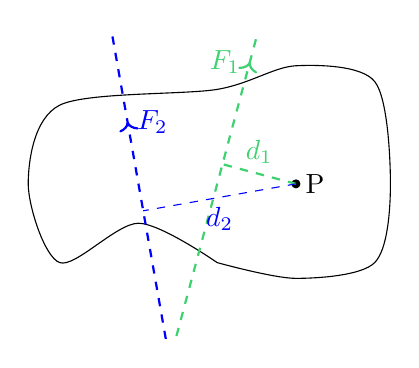
\begin{tikzpicture}
    \draw (0,0) coordinate (P)  node[right] {P};
    \draw[fill=black] (P) circle[radius=0.05, fill=black];
    \draw plot[smooth] coordinates { 
            (-1, -1) (-2, -0.5) (-3, -1) (-3.4, 0) (-3, 1) (-1, 1.2) 
            (0, 1.5) (1, 1.3) (1.2, 0) (1, -1) (0, -1.2)
            (-1, -1)
    };
    
    \draw[thick, dashed, color=ufogreen] 
        (-1,0)++(75:-2) coordinate (a1) -- coordinate[pos=0.9] (F1) ++(75:4) coordinate (a2);
    \draw[color=ufogreen] (F1) node[left] {$F_{1}$};
    \draw[thick, dashed, color=blue] 
        (-2,0)++(100:-2) coordinate (b1) -- coordinate[pos=0.7] (F2) ++(100:4) coordinate (b2);
    \draw[color=blue] (F2) node[right] {$F_{2}$};
    \draw [thick, color=blue, ->] (F2)++(100:-0.01) -- (F2);
    \draw [thick, color=ufogreen, ->] (F1)++(75:-0.01) -- (F1);

    \draw[thick, dashed, color=ufogreen]  (P) -- node[pos=0.5, above] {$d_{1}$} ($(a1)!(P)!(a2)$);
    \draw[dashed, color=blue]  (P) -- node[pos=0.5, below] {$d_{2}$} ($(b1)!(P)!(b2)$);
\end{tikzpicture}

Moment of a force: Torque.

In 3D the body and forces acting on the body are coplanar (always true in 2D),
the forces will tend to rotate the body about an
axis perpendicular to the plane. Then, by definition,
The moment of $\vec{F}$ about $P$ is $|\vec{F}| \times \text{perpendicular distance}$.

It is important to take into account
the direction of rotation: clockwise or anticlockwise.

If the body and forces acting on the body
and \emph{not} coplanar then different applied
forces will tend to \emph{rotate} the
body about different axes. Then,
we require a neater quantity to represent the
moment of a force.

$\vec{G}$ is the torque through a point $P$, and $\vec{F}$ is the force.
$d$ is the perpendicular distance from $P$ to the line of action of $\vec{F}$.

From diagram:
\[
|\vec{G}| = |\vec{F}| \times d
\]
$\vec{G}$ acts parallel to the axis of rotation.
This rotation is represented with the ???
of the vector cross product
\begin{equation}
    \vec{G} = \vec{r} \times \vec{F}.
\end{equation}
$\vec{r}$ is a position vector form $P$ to any point
on the line of action of $\vec{F}$.

\subsection*{Equilibrium}

For a body to be in equilibrium, we must have that
the sum of the vector moments of the forces
about any point is zero.

\begin{equation}
\sum\limits_{i}^{}\vec{G}_i = \vec{0} \equiv \sum\limits_{i}^{} \vec{r}_i \times \vec{F}_i = \vec{0}
\end{equation}

We can justify any point as follows:

Suppose the point under consideration is now $P'$ instead of $P$,
and let $\vec{a} = \overrightarrow{PP'}$. Then,
\[
\vec{r}_i \mapsto \vec{r}'_i = \vec{r}_i - \vec{a}.
\]
So, if we consider moments about $P'$,
\begin{align*}
    \sum\limits_{i}^{}\vec{G}_i &= \sum\limits_{i}^{} \vec{r}'_i \times \vec{F}_i\\
                                &= \sum\limits_{i}^{}(\vec{r}_i - \vec{a}) \times \vec{F}_i\\
                                &= \sum\limits_{i}^{}\vec{r}_i \times \vec{F}_i - \vec{a} \times\sum\limits_{i}^{} \vec{F}_i\\
                                &= \vec{0} - \vec{0} = \vec{0}.
\end{align*}

\subsection*{Couple}

Consider two forces $F_{1}$ and $F_{2}$ whose lines of action
are parallel and a distance $d$ apart,
where $F_{1}$ acts up and $F_{2}$ acts down.
Let $A$ a point on the line of action of $F_{1}$
and $B$ a point on the line of action of $F_{2}$ 
such that $AB$ is perpendicular to the lines of action of $F_{1}$ and $F_{2}$.

Let $Y,X$ be the resultant forces
perpendicular and parallel to $AB$, respectively.
Then we have $Y = F_{1} - F_{2}$, $X = 0$.

Take moments clockwise around $B$,
then we have $F_{1}d = Yx$.

So we have a non-zero resultant acting parallel to $F$,
at a distance $x$ from $B$.

The following is a special case of
above.

Suppose $F_{1} = F_{2} = F$, where $F \equiv |\vec{F}|$.
Then, the magnitude of the resultant, $F_{1} - F_{2}$, is now zero.

\begin{center}
    \begin{tikzpicture}
        \draw[->] (-1, -1) -- (-1, 1) node[left] {$\vec{F}$};
        \draw[dashed] (-1, 0) node[left] {$A$} 
            -- node[pos=0.5, above] {$d$} (1, 0) node[right] {$B$};
        \draw[->] (1, 1) -- (1, -1) node[right] {$-\vec{F}$};
    \end{tikzpicture}
\end{center}
However, the turning effect is \emph{not} zero.
A pair of equal and opposite parallel forces
is called a \emph{couple}.
In general, the sum of the moments of two forces
will depend on the point about which the moment
of the individual forces are taken,
but \emph{not} in the case of a couple.

\begin{center}
    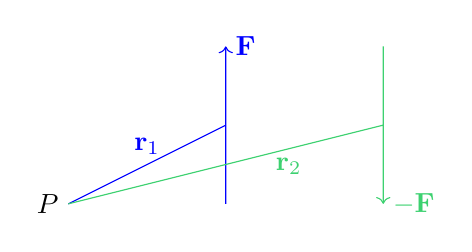
\begin{tikzpicture}
        \draw (0, 0) node[left] {$P$};
        \draw[->, color=blue] (0, 0) -- node[pos=0.5, above] {$\vec{r}_1$} (2, 1)
            (2, 0) -- (2, 2) node[right] {$\vec{F}$};
        \draw[->, color=ufogreen] (0, 0) -- node[pos=0.7, below] {$\vec{r}_2$} (4, 1)
            (4, 2) -- (4, 0) node[right] {$-\vec{F}$};
    \end{tikzpicture}
\end{center}

Taking moments about $P$:
\[
    \vec{r}_1 \times \vec{F} + \vec{r}_2 \times (-\vec{F}) = (\vec{r}_{1} - \vec{r}_{2}) \times \vec{F}.
\]
and thus does not depend on the choice of $P$.
Chooe $P = A$, then we have the moment $|\vec{F}|\times d$.

\subsubsection*{Characteristics of a Couple}
\begin{compactenum}
\item The linear resultant of a couple is zero.
\item The moment of a couple is non-zero and independent of the
    point the moment is taken about.
\end{compactenum}

\section{Centers of Mass}

Consider a solid body constructed
of many constituent particles.
The position of the center of mass (COM)
of the body is depends only on the 
mass and position of the constituent particles.
But, the location of the center of gravity (COG)
depends on the moment of the gravitational force
acting on each constituent particle.

If the gravitational force is uniform,
the COM coincides with the COG.

The reason that the COM is a useful concept
is because the total mass of the body
can be replaced bt a single mass at the position
of the COM with the total mass of the body.

For uniform bodies in $1,2,3$ dimensions, 
the COM usually resides within the body,
but it is not always the case.

\subsubsection*{Example}

Consider $N$ particles attached to a \emph{light} rod.

\begin{center}
    \begin{tikzpicture}
        \draw (-3,0) -- (3,0);
        \draw[->] (0,0) -- (0,2) node[above] {$R$};
        \draw (-3,0) node[draw, shape=circle, fill=black, inner sep=0.04cm] 
            {} node[below] {$P$};

        \draw[dashed] (-3,0) -- (-3, 1.5);
        \draw (-1.5, 1) node (d) {$d$};
        \draw[->] (d.west) -- (-3, 1);
        \draw[->] (d.east) -- (0, 1);

        \draw (0,0) -- (240:0.5) -- (-60:0.5) -- cycle;
        \draw (0,-0.4) node[below] {$Q$};

        \foreach \x in {-2, -1.2, 0.4, 1.7}
        \draw[ufogreen] (\x, 0) node[draw, shape=circle, fill=ufogreen, inner sep=0.04cm] {};

        \draw[ufogreen] (-2, 0)
            node[below] {$P_i$}
            -- (-2, 0.7) [dashed]
            ;

        \draw[ufogreen] (-2.5, 0.5) node[inner sep = 0.04cm] (di) {$d_i$};
        \draw[ufogreen, ->] (di.west) -- (-3, 0.5);
        \draw[ufogreen, ->] (di.east) -- (-2, 0.5);

    \end{tikzpicture}
\end{center}

Assuming that the system is in equilibrium, then
\begin{align*}
    \sum_{i}\vec{F}_i &= \vec{0} = m_{1}g + m_{2}g + \cdots + m_n g - R = 0 \\
                      &\sum_{i} m_i g = R\\
    \sum_{i} \vec{G}_i &= \vec{0} = d_{1}(m_{1}g) + d_{2}(m_{2}g) + \cdots + d_N(m_N g) - Rd\\
                       &\sum_{i} d_i m_i g = Rd
\end{align*}

Eliminating $R$ and $g$ from the equations yields
\[
d = \frac{\sum_{i=1}^{N} d_im_i}{\sum_{i=1}^{N}m_i} = \frac{1}{M}\sum_{i=1}^{N}d_im_i
\]
which is the position of the point where
the rod and masses balance 
just as if it was a single mass equal to the total mass
at the pivot.

Equivalently, taking moments at the pivot,
\[
\sum_{i=1}^{N}(d-d_i)m_i g = 0
\]
which can be rearranged to arrive at the same answer.

The position of the COM of a general multiparticle system
is given, by definition,
\[
\vec{R} = \frac{1}{M}\sum_{i=1}^{N}m_i \vec{r}_i
\]
where $M$ is the total mass of the system $\sum m_i$.
Note that the COM does not depend on the choice of origin.

\begin{center}
    \begin{tikzpicture}[scale=2]
        \draw[->] (0,0) node[left] {$O$}
            -- node[pos=0.5, above left] {$\vec{x}$} (2, 1)
            node[above right] {$C$};

        \draw (0,0) -- node[pos=0.5, below] {$\vec{d}$} (1.5, -0.5) [dashed]
            node [below right] {$O'$}
            -- 
            node [pos=0.5, right] {$\vec{x}'$}
            (2, 1);
    \end{tikzpicture}
\end{center}

So we have 
\begin{align*}
    \vec{R} &= M^{-1}\sum_{i=1}^{N} m_i (\vec{d} + \vec{r}'_i)\\
            &= M^{-1}\left(\vec{d} \sum_{i=1}^{N}m_i + \sum_{i=1}^{N}m_i \vec{r}'_i\right)\\
            &= \vec{d} + \vec{R}'
\end{align*}

\end{document}
